\documentclass[a4paper,11pt]{article}
\usepackage{amsmath}
\usepackage{amsfonts}
\usepackage{titling}
\usepackage{graphicx}


\newcommand{\WTF}[1]{\textbf{???}\textit{#1}\textbf{???}}
\newcommand{\?}[2]{#1\footnote{\textsc{Translator note}: #2}}
\newcommand{\nequ}[2]{\begin{align*}\tag{#1}#2\end{align*}}
\newcommand{\uequ}[1]{\begin{align*}#1\end{align*}}
\newcommand{\unit}[1]{\text{#1}}
\providecommand{\operatorfont}[1]{\texttt{#1}}
%\newcommand{\operatorfont}[1]{}
\newcommand{\grad}{\operatorfont{grad}}
\renewcommand{\div}{\operatorfont{div}}
\newcommand{\curl}{\operatorfont{curl}}
\newcommand{\rot}{\,\operatorfont{rot}\,}
\renewcommand{\exp}[1]{e^{#1}}
\newcommand{\pXpY}[2]{\frac{\partial #1}{\partial #2}}
\newcommand{\ppXpYY}[2]{\frac{\partial^2 #1}{\partial {#2}^2}}
\newcommand{\dXdY}[2]{\frac{d{#1}}{{d{#2}}}}
\newcommand{\ddXdYY}[2]{\frac{d^2{#1}}{d{#2}^2}}
\newcommand{\mf}[1]{\mathfrak{#1}}
\newcommand{\Nth}[1]{{#1}^\text{th}}

\newcommand{\citeauthor}[1]{\textsc{#1}}
\newcommand{\citetitle}[1]{\textit{#1}}
\newcommand{\citepub}[1]{#1}
\newcommand{\citevol}[1]{\textbf{#1}}
\newcommand{\citepage}[1]{#1}
\newcommand{\citedate}[1]{#1}
\newcommand{\citeyear}[1]{#1}

\newcommand{\El}[1]{\text{#1}}
\newcommand{\mnEl}[3]{{}^{#1}_{#2}{\El{#3}}}

\newcommand{\publication}[1]{%
    \gdef\puB{#1}}
\newcommand{\puB}{}
\renewcommand{\maketitlehooka}{%
    \par\noindent \puB}


\newcommand{\location}[1]{%
    \gdef\loB{#1}}
\newcommand{\loB}{}
\renewcommand{\maketitlehooka}{%
    \par\noindent \loB}

%\newcommand{\dX}[2]{\frac{d#1}{{#2}}}
%\newcommand{\dY}[1]{{d#1}}
%\newcommand{\pX}[1]{\frac{\partial{#1}}}
%\newcommand{\pY}[1]{{\partial{#1}}}

% \newcommand{\original}[1]{}
\newenvironment{translation}[0]{
}

\newenvironment{original}{
\renewcommand{\footnote}[1]{\small{(Footnote: ##1)}}
(\textit{Begin original text}:
}{
\textit{-- end original text})
}

\newenvironment{letter}[1]{
	\newcommand{\letternumber}{#1}
	\newenvironment{header}[0]{
		\newcommand{\from}[1]{\newcommand{\headerfrom}{####1}}
		\renewcommand{\to}[1]{\newcommand{\headerto}{####1}}
		\renewcommand{\date}[1]{\newcommand{\headerdate}{####1}}
		\renewcommand{\location}[1]{\newcommand{\headerlocation}{####1}}
		\newcommand{\note}[1]{\newcommand{\headernote}{####1}}
		\newcommand{\makeheader}{
		\begin{tabular}{|p{0.9\textwidth}|}
			\hline
			Letter \# \letternumber\\
			From: \headerfrom \\
			To: \headerto \\
			Date: \headerdate \\
			\ifdefined\headerlocation
				Location: \headerlocation \\
			\fi
			\ifdefined\headernote
				Notes: \headernote \\
			\fi
			 \hline
		 \end{tabular}\\
		}
	}{

	}
	\renewcommand{\d}[1]{d##1}
	\newcommand{\figw}[2]{
		\begin{figure}[h]
			\begin{center}
			\includegraphics[width=##2]{##1}
			\end{center}
		\end{figure}
	}
	\newcommand{\fig}[1]{\figw{##1}{150pt}}
	
}{
 \quad  \\------------------------------------\\
}
%new environment, define _ to append to denom and ^ to append to num
%in after, \frac{\num}{\den} — _/^ should be undefined automatically

%\providecommand{\n}{}
%\providecommand{\d}{}
%\newcommand{\numer}{}
%\newcommand{\denom}{}
%
%\newenvironment{derivative}[1]{
%	%\renewcommand{\numer}{}
%	\renewcommand{\n}[1]{\let\numer{\numer #1##1}}
%	%\renewcommand{\denom}{}
%	\renewcommand{\d}[1]{
%		\let\ndenom{\denom #1##1}
%		\renewcommand{\denom}{\ndenom}
%	}
%}{
%\numer\\
%\ensuremath{\frac{(\numer)}{(\denom)}}\\
%\denom\\
%}
%
%\newcommand{\D}[1]{
%\begin{derivative}{d}
%	#1
%\end{derivative}
%}

\newcommand{\D}{\mathrm{d}}

\newcommand{\derX}[2]{
\renewcommand{\dY}[1]{\ensuremath{\frac{#1 #2}{#1 ##1}}}
\renewcommand{\pY}[1]{\dY{##1}}
}

\newcommand{\dderX}[2]{
	\renewcommand{\dY}[1]{
		\renewcommand{\dY}[1]{
			\ensuremath{\frac{#1^2 #2}{ {#1 ##1}\, {#1 ####1}}}
		}
	}
	\renewcommand{\ddY}[1]{
		\ensuremath{\frac{#1^2 #2}{{#1^2 ##1}}}
	}
	\renewcommand{\pY}[1]{\dY{##1}}
	\renewcommand{\ppY}[1]{\ddY{##1}}
}

\newcommand{\dY}[1]{\text{ERROR: dY without dX}}
\newcommand{\pY}[1]{\text{ERROR: pY without pX}}
\newcommand{\ddY}[1]{\text{ERROR: ddY without ddX}}
\newcommand{\ppY}[1]{\text{ERROR: ppY without ppX}}
\newcommand{\ddX}[1]{\dderX{\D}{#1}}
\newcommand{\ppX}[1]{\dderX{\partial}{#1}}
\newcommand{\dX}[1]{\derX{\D}{#1}}
\newcommand{\pX}[1]{\derX{\partial}{#1}}

\begin{document}


%\D{\n{a}\n{b}\d{x}\d{y}}

\begin{letter}{1}

\begin{header}
\from{Weyl}
\to{Pauli}
\date{1919/05/10}
\location{Zurich}

\makeheader

\end{header}

Very honorable Herr Pauli!

It brings be extraordinary joy to be able to greet you as a coworker. How you have somehow managed, at such a young age to set yourself up in possession of all the means of knowledge, and to gain the freeness in ideas that is essential to make the relativity theory your own, is nearly incomprehensible to me.

I have recently received proofs of the third edition of my book I have briefly, \?{after which I wrote to Herr Dr Thirring}{nachdem ich Herrn Dr Thirring schrieb} (they were only provisionally set; when it will be printed and published is still undetermined). I sent the proofs to Herr Thirring, which contain what I believe to be the final version of the "pure infinitesimal geometry", and the conclusion of the book, which treats its physical meaning (electricity and gravitation). Unfortunately I can only spare one copy; but I assume that you could easily get ahold of the proofs from Herr Dr Thirring if you want to see them.

In it I believe, the question as to what quantities are to be introduced in an arbitrary action principle as the current and energy-momentum is clearly answered. I have naturally in no way overlooked the invariants you specified; indeed one first runs into them \?{when starting with the Einstein theory}{wenn man von der Einsteinschen Theorie herkommt}. To the four you mentioned I add a fifth, $R_{iklm}R^{ilmk}$. Can every \?{rank-2 quadratic invariant}{quadratisch aufgebaute Invariante vom Gewichte-2} formed from the curvature components $R$ be \?{put together from linear combinations}{linear...zusammensetzen} of these 5? I have not explicitly proven it; but the question can certainly be easily decided, with some expenditure of calculations. \WTF{A.a.O} I also directly consider the invariant $R^2$; I find there that one inevitably arrives at the cosmological term. You will find the remarks about the normalization $R=\text{const}$ in harmony with those in yours. \?{Setting up the mechanical equations for a material particle has given me many headaches}{Viel Kopfzerbrechen hat mir die Aufstellung der mechanischen Gleichungen für ein materielles Teilchen bereitet}. To get clarity there, I first had to put aside the investigation of the action principle $R_{iklm}^{iklm}$ and instead of this I have attempted on the one hand to draw totally general valid consequences of my theory, on the other hand to discuss that in the easiest way and \?{present the connection to the $R^2$ that is immediately apparent in Maxwell-Einstein}{den Anschluß an Maxwell-Einstein unmitte lbar darbietende $R^2$ vorgenommen}. So there I touch on your results in part. In the paper in Annalen der Physik I have also formulated the electron problem for just this simplest case, without being able to solve it (I have not yet worked out the elimination like you did it: to a single 3rd-order equation — even if I reduce the problem from 4th- to 3rd-order by quadrature).

Only publish your results in the form that seems appropriate to you; a collision in one point or another is in the end not a disaster. I still haven't yet received any proofs of the Annalen paper; who knows when it will be published! But it contains beyond that what I started in the last chapters of the book, only with the formulation of the electron problem.

To the question of the \?{asymmetry}{Ungleichwertigkeit} of positive and negative electricity, I say this: if the invariant entering into the action variable is \?{formed rationally}{rational...gebildet} from the $g_{ik}$, $\varphi_i$ and their derivatives, then the charge of a body is determined independently of any mass unit, incl the sign, so far as the world tube swept out by the body has a distinguished past $\to$ future sense. The asymmetry in electricities would also lead to an asymmetry past and future, which of course is not expressed in the "\?{laws of nature}{Weltgesetzen}". But how this problem is to be solved, we currently have no idea. I hold that is in no way excluded that in matter there is something fundamentally different than mere "knots" of gravi-electromagnetic fields. You must not think me such a dogmatist that I would believe now the Philosopher's Stone has finally been found. — If one also takes action invariants into consideration that are not \?{rationally formed}{.}, but rather something with a square root, then the asymmetry of the electricities also naturally emerges independently from past and future.

I unfortunately have to more \?{prints}{Separata} of my paper in the Berliner Berichten (they are out of print); per your request I have set aside the one published in the Zeitschrift für Mathematik, though I would now prefer to put it aside in favor of the improved version in the 3rd edition of Space-Time-Matter.

It would make me very happy if the road of your studies should sometime take you to Zurich. If you want to come to Switzerland now, it would not be, I think, too difficult \?{to provide you with the travel documents}{Ihnen von hier aus die Einreisebewilligung zu verschaffen}.

With best wishes,

H. Weyl

\end{letter}
\begin{letter}{2}
\begin{header}
\from{Weyl}
\to{Pauli}
\date{1919/12/09}
\location{Zurich}

\makeheader

\end{header}

Very honorable Herr Pauli!

Many thanks for the \?{proofs}{Korrekturbogen} and your paper from the Physikalische Zeitschrift! Please don't take my silence too badly. Written correspondence with people is grueling for me; lately I have been with completely different things, logical foundations of analysis, and am impeded by shaky health.

Regarding your result that the Einstein field of a "point mass" is also a rigorous solution of the field equations associated with the action quantities $R_{iklm}^{iklm}$, I am naturally pleased. — I likewise find the \?{over-determination}{Überbestimmtheit} of the static field more pleasant than alarming. I find that only the \textit{static, spherically-symmetric} has a physical meaning (an actually static solution can only be spherically symmetric), and so the over-determination vanishes. It seems to me that nothing else is to be expected with rigorous field equations. The essential difference between the two electricities can emerge in Mie's theory via a root, e.g. $\sqrt{\varphi_i \varphi_i}$ in this way: if there are any roots in the static case, according to the principle of analytic continuation, $\varphi_0$ \textit{and not $=|\varphi_0|$} (I assume $ds^2 = dx_0^2 - dx_1^2 - dx_2^2 - dx_3^2$). In a non-static field deviating little from that, it is impossible for $\varphi_i\varphi^i >0$ everywhere; that must be discussed in more detail. In any cade, with many-valued functions in the action principle a single analytic branch among these is understood, the selection of which \textit{cannot} be done in a coordinate-free manner. Why should that be excluded in my theory? But we are now ignoring just such a many-valuedness! If we have an isolated system that sweeps out a world-tube, then its charge $e$ equals the flux of the vector density $\mathcal{E}_i$ through an arbitrary cross-section $S$ of the tube:

%\fig{02-19191209-01}

\begin{figure}[h]
	\begin{center}
	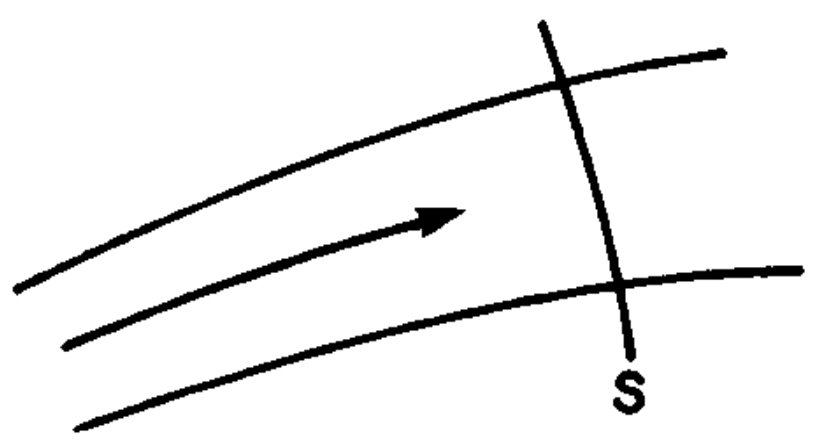
\includegraphics[width=150pt]{02-19191209-01}
	\end{center}
\end{figure}

$e$ is an absolutely definite number as soon as a flow direction (past $\to$ future) is fixed in the tube. That is what I meant with my assertion that the sign of the charge is dependent on the distinction between past and future. I hold, as opposed to most physicists, their essential difference to be a fact of much more fundamental significance than the essential difference between positive and negative electricity. Nevertheless, modern physics is right that it has no place in "laws" or "field physics". \?{I am then firmly convinced that statistics are fundamentally independent with regards to causality, which is a "law"; while it is just absurd to suppose a continuum as something pre-existing}{Denn ich bin fest überzeugt davon, daß die Statistik etwas prinzipiell selbstständiges gegenüber der Kausalitat, dem "Gesetz" ist; weil es übberhaupt widersinnig ist, sich ein Kontinuum als etwas fertig-Seiendes vorzustellen}. Field theory, I think, really only plays the role of "world geometry"; in matter there is still something else, something real, that is not causally interpretable, but rather perhaps can be thought of under the concept "independent decisions", and which we treat in physics through statistical calculations. It is quite possible that we must must leave the essential distinction between past and future, between positive and negative electricity here; that it will then still find no place in field theory. These are \textit{suggestions} whose more detailed investigation would take too much space.

I am in agreement with you that the legitimacy of speaking of a conservation law $\pXpY{\gamma_i^k}{x_k} = 0$ as an energy-momentum law must be disproven by the fact that for a material particle it yields the mechanical equations. Your derivation of the same shared in your last letter however did not seem as compelling to me.

That the fields inside the electron cannot be measured, one can probably only say: differences inside the electron could never \?{causally create}{kausal bedingen} such changes in the course of the world which grow to an immediately-perceptible magnitudes. Namely, as soon as such effects occur, I can use them to "measure" any interior differences. But why should that not happen! I believe e.g. that the circumstance that electron does not radiate in the stationary Bohr orbits, is a sign of an inner change in the electron arising through the acceleration that allows it to keep its energy; then why should it behave like a rigid sphere with rigid charge even with non-quantized acceleration?

With best thanks and greetings, yours faithfully

H. Weyl



\end{letter}

\begin{letter}{3}
\begin{header}
\from{Pauli}
\to{Land\'e}
\date{1919/12/18}
\location{Munich}

\makeheader

\end{header}

Very honorable Herr Doktor Land\'e!

On behalf of Herrn Geheimrat Sommerfeld I have studied your paper on the reflections on the interactions of circular orbits in their quantization by means of the adiabatic hypothesis in more detail. I have found that the goal can be reached much more simply if, one doesnt take the kinetic energy as a function of $a$ from the equilibrium condition likeyou do, but rather introduces the angular momentum and instead write the equilibrium condition in the Hamiltonian in the Lagrangian form
\nequ{1}{
H_k(p_k, a_k)= \frac{p_k^2}{2ma_k^2} + U_k\\
\pX{}\pY{a_k}\left(H_k + \sum\limits_{j\neq k}V_{jk}\right)=0.
}
Your condition
\nequ{3}{
\D{W_k} + \pX{}\pY{a_k}\left(\sum\limits_{j\neq k}V_{jk}\D{a_k}\right) = 0
}
then says nothing more than the adiabatic invariance of the angular momentum. Namely
\uequ{
\D{W_k} = \D{H_k} = \pX{H_k}\pY{a_k}\D{a_k} + \pX{H_k}\pY{p_k}\D{p_k},
}
so as a consequence of (1)
\uequ{
\D{p_k} = 0.
}

Hence it requires longer investigation as to whether your equation (3) is integrable. On the contrary one is led immediately to Sommerfeld's rule which is also justified from the standpoint of the adiabatic hypothesis here: the \WTF{Ringradien} from the equilibirium condition (1) are used as angular momenta $p_k$ and are set equal to the unperturned values, i.e. equal to $n_k\frac{h}{2\pi}$.

With best greetings yours faithfully,

Pauli
\end{letter}
\begin{letter}{4}
\begin{header}
\from{Born}
\to{Pauli}
\date{1919/12/23}
\location{Frankfurt}


\makeheader

\end{header}

Very honorable Herr Pauli!

My answer do Enwald, which has probably been shown to you, will probably already have shown you that I have very much enjoyed your contribution. I have already applied \?{your method}{die von Ihnen gebrauchte Umsummierung} for the case of \?{surface energy}{Oberflächenenergie} (capillarity constant) myself, but did not notice that it can even be found for the tension components. With your permission, I will include this consideration in the encyclopedia article; but do you not want to publish something brief somewhere>

I have read your paper in the new issue of the Proceedings of the German Physical Society on the Weyl theory with great interest; however I am momentarily not totally \?{up to speed with}{bin...in...zu Hause} the relativistic formulae, since I haven't thought about it in a month, but I understood the idea of your observations. I was especially interested in your remarks at the end, that you hold that applying continuum theory inside the electron to be meaningless, since there it is dealing with in-principle unobservable things. I have pursued exactly this idea for a long time, but up to now without any positive results, namely, that the way out of all quantum difficulties must be sought totally \?{theoretical}{prinzipiellen} points: one cannot carry over the concept of space and time as a 4-dimensional continuum from the world of macroscopic experience, this apparently demands another type of \WTF{numeric manifold} as an adequate basis. But. how that would be made, I have no inkling. Though I am not old, I am too old and weighted down to have something like that occur to me. That is your task; from all I have heard of you, you are made for such problems.

If however you want to wander around the lowlands of the usual physics for the present, I recommend a problem to you that was taken up in a paper by Stern and me that just came out, which I am sending you simultaneously. One should show that the surface energy of the cubic surfaces of NaCl crystals (in vacuum at absolute zero) is smaller than that of any other surface. The problem requires, I believe, a rather deep study of \?{the potentials at half-lattice points}{der Potentiale von Halbgittern}; there one could perhaps take advantage of Ewald's method. I must however confess that I have always found Madelung's procedure for calculating lattice potentials to be more convenient and more intuitive.

I would be very glad if you could visit us here sometime or even one day work with us. \?{Even if all connections are closer here like in Munich}{Wenn auch alle Verhältnisse hier enger sind wie in München}, we still have some specialties of different types than they do.

With warm greetings to Sommerfeld, Ewald and all the other colleagues.

Very faithfully yours

M. Born

\end{letter}
\begin{letter}{5}
\begin{header}
\from{Pauli}
\to{Oppenheim}
\date{1920/05/07}
\location{Munich}
\note{Carbon copy}

\makeheader

\end{header}

Very honorable Herr Professor!

Herr Geheimrat Sommerfeld has conveyed to me your desire to learn about the article on relativity theory from the Physics volume of the Encyclopedia, and so I share its status with you:

I. Critical discussions on the foundations of the special theory of relativity.

II. Mathematical aids (tensor calculus, variation laws).

III. Further extensions of the special theory of relativity (applications to electrodynamics, mechanics, etc).

IV. Foundations of the general theory of relativity. (Equivalence hypothesis, generality of the behavior of measuring sticks any clocks, motion of point masses and light rays, influence of gravitational fields in material processes.)

V. Einstein's field equations of gravity and their consequences.

VI. Cosmology.

VII. Theories on the nature of the electric elementary particles. (Poincaré, Mie, Weyl, Einstein.)

A collision with Herrn Kottler's article, with discussion of the general foundations of the theory of relativity can hardly be avoided, on the other hand an agreement can be made on the following points: a) I had the intention to explain in rather more detail the attempt by Poincaré et al to arrange gravitation under the special theory of relativity. But since according to your information Herr Kottler will treat it anyway, I will be brief. b) I would like to ask whether Herr Kottler will also mention the Nordstrom theory. It would suffice if in the two articles there was about an hour. I would like to coordinate with Herrn Kottler this.

c) Also as regards Einstein's cosmological observations, a division of labor can perhaps be reached.

It would perhaps be good if the same notation could be used in both articles and I would like to make the following proposals there:

1) Give the line element $\D{s}^2$ in the general theory of relativity 3 positive and 1 negative (and not, like many authors do, 1 negative and 3 positive) signs.

2) Denote the coordinates by the Hessenberg notation with $x^1,\dots,x^4$ (instead of with $x_1,\dots,x_4$)

3) Instead of $\left\{{}^{rs}_{i}\right\}$ and $\left[{}^{rs}_{i}\right]$ always write just $\Gamma^i_{rs}$ and $\Gamma_{i,rs}$ and always call these quantities the geodetic components (of the associated coordinate system). 

I would ask you to share these proposals with Herrn Kottler, it would probably be best if I can then \?{come to an agreement}{mich...ins Einvernehmen setze} with him directly.


\end{letter}
\begin{letter}{6}
\begin{header}
\from{Pauli}
\to{Land\'e}
\date{1920/05/12}
\location{Munich}

\makeheader

\end{header}

Dear Dr Land\'e!

With the approval of Geheimrat Sommerfeld I would be free to share with you my views on the inertia of potential energy that you have postulated. I start from the fact that the equations of motion must read in every case

\nequ{1}{
\dX{}\dY{t}\frac{m_0 \vec{r}}{\sqrt{1-\frac{v^2}{c^2}}} = 
e\left(\vec{E} + \frac{1}{c} [\vec{v}\, \vec{H}]\right).
}
Any inertia of the potential energy must then be caused by a deviation of the electromagnetic field from the Coulomb field. First a magnetic field is present and second instead of the Coulomb, calculating with the \textit{retarded} (four-)potential. The calculation (which incidentally Herr \textit{Fokker} has carried out in detail, to be published shortly in the Archive Néerlandaise) shows that the matter is not at all as simple as you assume. There is indeed a term on the right side with $\ddot{\vec{r}}$, but this does not have the same form as the term that is given by your Ansatz. As far as I see, that is connected with the circumstance that at no moment do the electrons move in parallel, as is the case with the \textit{additional} velocities of the electrons with a \WTF{Gesamttranslation des Ringes}. If an \textit{external} force acts on the whole ring, the calculation with the retarded potentials must naturally lead to the inertia of potential energy, at least ignoring additional terms of higher order. — Here the principle difficulty is still present, that one never knows how far classical mechanics is correct. If one were to calculate totally consistently according to the classical scheme, then one would naturally arrive at radiation in the static orbits. My view is then, briefly summarized, the following: the theory of doublets is to be improved by considering the retardation. Any inertia of the potential energy \textit{is likewise caused by the retardation} and would already be taken into account with it. The calculation shows however that your simpler Ansatz is incorrect and has to be replaced by much more complicated one.

I again thank you for sending your offprint, and remain

Yours very faithfully

Pauli
\end{letter}
\begin{letter}{7}
\begin{header}
\from{de Sitter}
\to{Pauli}
\date{1920/05/25}
\location{Arosa}

\makeheader

\end{header}

Very honorable Herr Doktor!

Many thanks for your interesting papers. Pre-prints of my papers are being sent to you from Leyden. Allow me to draw attention to two points — though of secondary interest — which are not in my printed papers, or are only raised in footnotes.

1. The $\lambda$-term introduced by Einstein now seems to be generally called the "cosmological term". That is wrong. It has nothing to do with cosmology. True, Einstein's treatment of cosmological considerations where he introduced it started with a mention of a cosmological problem; but, as I have shown, that problem is \textit{not} solved by $\lambda$, not even touched upon. If $\lambda$ is to be given a name, call it the \textit{inertial flux}, or inertial coefficient, since it serves to make the inertia relative. Inertia has nothing more or less to do with cosmology than e.g. gravitation, or light or magnetism.

2. In the same treatment Einstein has assumed a finite space of constant positive curvature for the three-dimensional physical world. There are two of these: the elliptic (simple-elliptical) and the spherical (double-elliptical). In almost all papers the second is discussed, yet the \textit{first}, the \textit{simple-elliptical}, is the simpler and more natural. The spherical space is only a totally unnecessary doubling of it.

Our usual Euclidian geometry is the limiting case of the elliptical, not the spherical case. Since a line has a point at infinity, a plane a line, two lines cannot cross at more than \textit{one} point (at infinity or not), and finally the paradox that in the elliptical space a plane is \textit{one}-sided exists in our Euclidian geometry too: if we go along a branch of a hyperbola, we come back to the other branch, and indeed on the other side of the asymptote (or any other line) without having to cross the asymptote. If one wants to come back to the same side of the asymptote, then the trip must be made twice.

Faithfully yours,

W. de Sitter

\end{letter}
\begin{letter}{8}
\begin{header}
\from{Schr\"odinger}
\to{Pauli}
\date{1920/07/12}
\location{Jena}

\makeheader

\end{header}

Dear Herr Pauli!

Many thanks for your letter. I am glad to hear that are paying attention to the poor, long-neglected magnetism and have put beautiful results about it within reach, and also glad that we have come to an understanding, since it would be madness to work in parallel and on top of one another now, when the field \WTF{in Modellangelegenheiten} is truly large enough to, on the contrary, to make the most parsimonious \textit{division of labor} a pressing demand. Since the matter however has not stopped being very compellingly interesting to me, I would be very thankful to you if you would be able to make it possible for me  to get a proof of your relevant paper as soon as possible — in the present \?{conditions of publication}{Publikationsverhältnissen} it otherwise takes far too long to be able to eventually include further reflections, and life is short.

I am very curious on your diamagnetic note. Namely it seems to me that e.g. in helium the Bohr orbits are not at all sufficient for explaining the relatively strong diamagnetism ($\kappa = -11\cdot 10^{-9}$), even if it is not partially obscured by a (of course very weak) orientation effect. So the diamagnetism might be in part a nuclear effect, which would be quite interesting — it would then, assuming sufficiently precise measurement, provide alongside gravitation and radioactivity a third means of distinguishing isotopes.

That the \WTF{Kreiselmodell} should \textit{not} give the Curie law would astonish me, and I cannot quite believe this result, that you yourself only expressed with great reservations. — For me, a great difficulty in the \textit{Kreiselmodell} lies in the following. I will call the motion \textit{without} an $H$-field a \WTF{Thermopräzession}, the aperture angles are then "quantized" in the well-known manner. The moment \textit{in the direction of the field}\footnote{therefore the cosine of the field direction-axis of thermal precession angle.} however should, according to Epstein (Physikalische Zeitschrift \textbf{20}, 291, 1919) be quantized \textit{only when} the field lies \textit{inside} the cone of thermal precession. I cannot believe that, though I acknowledge the formal basis, which you among others \?{have found questionable}{auseinandergesetzt finden}.

Also the exclusion of \WTF{states with magnetic axis $\perp$ field through Bohr} seems somewhat dubious to me. With only \textit{one} quantum that would mean a full orientation of the axes, already in the weakest field, and almost half \textit{in the field direction}, half $\perp$ to it. That would have to produce a strong \WTF{, auch anderweitig, }e.g. electrically or optically perceptible anisotropy and even in the weakest field, as mentioned, "proportional to the zeroth power" of the field strength. That contradicts physical \?{intuition}{Gefühl}.

Finally, as to the molecule with magnetic axis $\perp$ the binding line of the nucleus, I have also already thought about that. I hold such a model to be unlikely, since I believe that I can show that the electron angular momentum in thermal motion would suffer constant continuous changes of its own order of magnitude. If you consider the 4 vectors $\vec{J}_e$ (electron momentum), $\vec{J}_k$ (nuclear momentum from thermal motion), $\vec{J}$ (total momentum), $\vec{r}$ (radius vector of a nucleus from the center of mass). It is $\vec{J} = \vec{J}_e + \vec{J}_k$, since e.g. "electron momentum from thermal motion" can be ignored. 

\begin{figure}[h]
	\begin{center}
	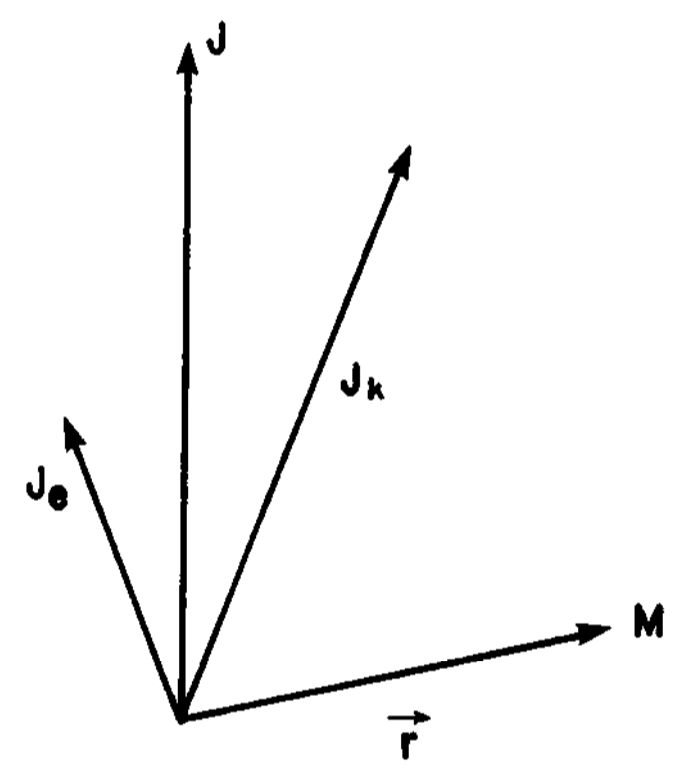
\includegraphics[width=150pt]{08-19200712-01}
	\end{center}
\end{figure}

Now $\vec{r} \perp \vec{J}_k$ (since $\vec{J}_k = 2M[\vec{r}\, \dot{\vec{r}}$) and $\vec{r} \perp \vec{J}_e$ (by assumption), so $\vec{r}\perp\vec{J}$ as well. But then the nuclear motion could only exist in a track around the invariable axis, so $J_e$ must also have this direction. Yet that cannot always be the case.

If these remarks have a big hole in them, please don't embarrass me in front of other people; but I think that it stands up well. — Indeed, the $\El{H}_2^+$ must be calculable ala Jakobi. Only working out every single possibility is so wearisome that without further clues, I don't want to poke around with it much.

Warmest greetings — faithfully yours,

Schr\"odinger

\end{letter}
\begin{letter}{9}
\begin{header}
\from{Schr\"odinger}
\to{Pauli}
\date{1921/02/13}
\location{Stuttgart}

\makeheader

\end{header}

Dear Herr Pauli!

Also for your \?{suggestion}{Anregungen}, I thank you very much. The difficulties that you mention of course \textit{exist}. Yet the following \WTF{Verse} can be made of them.

The non-existence of the circular orbit $n=1, n'=0$ \?{would line up with the fact that}{wäre in Parallele zu setzen damit} (according to Land\'e, Zeitschrift f\"ur Physik \textbf{2}, 87, 1920) with alkaline \textit{ions} the elliptical, \textit{not} the circular shell is built out. Perhaps the outermost system falls out to the elliptic state because of this elbow room. In any case \textit{if} my hypothesis is correct at all, then, \WTF{wegen der Stetigkeit des Anschlusses von $\frac{3}{2}S$ an $\frac{5}{2}S$ \dots}, the normal orbit must be my lowest orbit $n=1$, $n'=1$, or eventually even $n=1$, $n'=2$ and no other. At least with the alkali. With the alkaline earth metals the normal orbit is $\frac{3}{5}S$ (\?{singlet lines}{Einfachlinien}). Here a "jump" \WTF{gegen} $\frac{5}{2}S$ etc seems to actually be present (if I understand \textit{Dunz} correctly). \?{It can perhaps touch on the fact that}{Er kann vielleicht daher rühren, daß} at $\frac{3}{2}S$ the two electrons run in a "\WTF{Biellipsenverein}" (I mean both symmetric to the nucleus in the type of orbit I worked out), at $\frac{5}{2}S\dots$ on the other hand only \textit{one} of them is lifted out. For the alkaline earth triplets I would let \textit{one} electron lie in the circular orbit ($n-1,n'=0$) — indeed there is no longer complete freedom — the \textit{other} I would let run through an orbit of the new type. Basically, triplet terms and singlet terms would be distinguished by the distinguishable behavior of the \textit{second} electron and thereby very naturally explains the occurrence of \textit{two} \WTF{Seriensysteme} rather than a single one.
Naturally that all needs calculation, which unfortunate;y because of the ignored perturbations still can only yield very qualitative results. I have not even worked out the alkaline earth doublets yet. In the absence of my wife, who had to accompany my mother to Vienna, I am presently running "my own kitchen" and that takes up rather much time.

I must have a look at the situation with the Roentgen doublet. Land\'e's \WTF{Ellipsenvereine}, which probably come into play there for the $L$-shell, \?{have the irksome property that the high (cubic-)symmetry only sets in secularly through the relativistic perihelion precession}{haben das lästige, daß sich die hohe Symmetrie erst säkular durch die relativistische Perihelwanderung einstellt}. They correspond - somewhat - to spherical shells that \textit{pulsate} and simultaneously make \?{flattening vibrations}{Abplattungsschwingungen} wherein the pulsation frequency and flattening frequency are slightly different, so that "beats" occur; e.g. the strongest flattening or the spherical form happens together now at the stage woth the highest, now at the stage with the lowest volume. (The flattening takes place in quick succession on the three coordinate directions.) Replacing this object by uniformly pulsating spherical shells is even less permissible than the shell with circular orbits. \WTF{Oder ist das schon gehupft wie gesprungen?}

Warmest greetings, faithfully yours,

Schr\"odinger

\end{letter}
\begin{letter}{10}
\begin{header}
\from{F. Klein}
\to{Pauli}
\date{1921/03/08}
\location{G\"ottingen}

\makeheader

\end{header}

Dear Herr Pauli!

Your parcel has arrived here correctly and I thank you and Sommerfeld for it. and declare myself in agreement with this Modus procedendi. So I have written directly to Teubner that he is to begin with the essay, also gave him the desired instructions on mailing the proofs. Hopefully that also has \?{helpful}{fördernden} influence on Kottler's paper.

My own papers have no speculations on natural philosophy, but rather only the flow of the path of mathematical ideas, which appeared to me with Laue e.g. often as very tortuous and inscrutable. I like to mention that Einstein wrote me in this manner on my third note: he felt himself lucky, like a child who has been given chocolate bar by his mother (Einstein is always so charming in his personal correspondence, in total contrast to the \?{foolish reports put out to honor him}{törichten Reklamatum, das ihm zu Ehren in Bewegung gesetzt wird}). Another item that I have particularly attempted to make clear in my lecture issues is the historical facts of the matter. It is true that Poincare's first note in the Comptes Rendus 140 preceded Einstein and additionally (in Rendiconti di Palmero) first showed that Lorentz had a \textit{group} of transformations. From then on a contrast, that alone makes it comprehensible that Poincare, in his 1911 G\"ottingen lecture "sur la nouvelle mécanique" does not mention the name Einstein at all. I would hold that it is important that such and similar facts come our of your article. There is still enough left over for Einstein.

You could otherwise leave my issue so long that the entire work of the encyclopedia article is taken up by it. \?{Perhaps it is even more important than it was with me to consult the Dutchman on certain questions}{Vielleicht sollten noch stärker, als es bei mir geschehen ist, betreffs der Einzelfragen die Holländer herangezogen werden}. I have long been hindered by the unaccustomed language, since I only have the original, written in Dutch, at hand.

Another much simpler matter. After Batemann had drawn attention to the fact that the Maxwell equations \?{go over into themselves}{in sich übergehen} with his $G_{15}$, it is clear from E Noether's laws that it gives 15 divergence relations for the named equations. This had been meanwhile explicitly worked out by one of my students, Dr Bessel-Hagen, who found some relations that were unknown in the contemporary literature. But, before I take it to the Mathematischen Annalen, I would like to first have the physics part \?{checked}{kontrolliert}. Dr Bessel-Hagen has just traveled to Berlin for the holiday (Address Berlin W, Kurfürstendamm 200), and I advised him to use his personal connections to prepare the Planck section. Perhaps it would also be useful if he made personal contact with you. I would also like to inquire whether you have anything to say on this question, \?{i.e.}{ev.} whether I should request Bessel-Hagen to contact you.

Unfortunately I myself cannot go any further into these things now. I have to prepare the second volume of my collected works and accordingly I am deep in the theory of algebraic equations.

Best greetings, faithfully yours,

Klein

\end{letter}
\begin{letter}{11}
\begin{header}
\from{F. Klein}
\to{Pauli}
\date{1921/04/28}
\location{G\"ottingen}

\makeheader

\end{header}

Dear Herr Pauli!

Generally I would ask you to check whether the presentation is sufficiently clearly-written and orderly for the reader. Naturally you know these things from personal experience in Sommerfeld's seminar, which cannot be assumed of the reader and perhaps has given rise to occasional vagueness of expressions (which does not disturb daily intercourse). 


Best greetings, yours faithfully,

Klein

...In general I would say, one should now present the thing partially from the standpoint of the new theory and only over say afterwards how complicated, e.g. unsymmetric the things came out earlier. The other way around, where the reader always expects to just work from the incomplete version through to the improved one, made 
 book so unbearable. Your presentation is already much more \?{to my taste}{in meinem Sinne}...

\end{letter}

\end{document}